\section{Zdroj napětí}
\indent\indent Pro napájení jednotlivých bloků je potřeba zajistit tři napětí a to o hodnotě $+5~V$, $-5~V$ a $+12~V$. Toto zabezpečuje zdroj realizovaný pomocí dvou transformátoru  TR1 a TR2.

Transformátor TR1 má symetrické vinutí, které je zapojeno do série. Krajní vývody těchto vinutí jsou připojeny na dvoucestný usměrňovač realizovaný Graetzovým můstkem . Filtrační kondenzátory jsou pak připojeny z kladného a záporného pólu usměrňovače proti střednímu vodiči, který vznikl spojením vinutí transformátoru. Z takto připraveného symetrického napětí jsou pak napájeny integrované stabilizátory 7805 a 7905, na jejichž výstupech jsou stabilizovaná napětí $\pm5~V$.

Zdroj $+12~V$ je tvořen transformátorem TR2 Graetzovým můstkem D1, filtračním kondenzátorem C3 a stabilizátorem 7812 (U3). Pro ochranu stabilizátoru je použito přemostění diodami D3, D4 a D5.



\begin{table}[H]
	\begin{center}
		\caption{Tabulka použitých součástek pro desku zdroje}
		\label{tab:zdroj_os}      
		\begin{tabular}[H]{!{\vrule width 1pt}c|c|c|c!{\vrule width 1pt}}
		    \specialrule{1pt}{0pt}{0pt} 
		    \textbf{Určovatel}	&	\textbf{Pouzdro}	&	\textbf{Množství}	&	\textbf{Určení}	\\\specialrule{1pt}{0pt}{0pt} 						
			C1,C2,C3	&	Elko\_vert\_25x12.5mm\_RM5	&	3	&	470u/100V	\\\hline
			C4-C9	&	C\_0805	&	6	&	100n	\\\hline
			D1,D2	&	bridge\_DFM	&	2	&	DB104	\\\hline
			D3,D4,D5	&	diode\_do41	&	3	&	D\_Schottky	\\\hline
			F1	&	fuse\_socket	&	1	&	32mA/230V	\\\hline
			M1	&	M3	&	1	&	M3	\\\hline
			P1	&	SolderWirePad\_single\_2mmDrill	&	1	&	L1	\\\hline
			P2	&	SolderWirePad\_single\_2mmDrill	&	1	&	L2	\\\hline
			P4	&	SolderWirePad\_single\_2mmDrill	&	1	&	N1	\\\hline
			P5	&	SolderWirePad\_single\_2mmDrill	&	1	&	N2	\\\hline
			P6-P11	&	vasch\_strip\_3x2	&	6	&	MLW6	\\\hline
			T1	&	BV\_EI\_382	&	1	&	TRANSFO2	\\\hline
			T2	&	BV\_EI\_303	&	1	&	TRANSFO	\\\hline
			U1	&	LM78XXV	&	1	&	7805	\\\hline
			U2	&	LM79XXV	&	1	&	7905	\\\hline
			U3	&	LM78XXV	&	1	&	LM7812	\\\hline
			P3	&	CON\_EU\_PANEL	&	1	&	CON\_EU\_PANEL	\\\specialrule{1pt}{0pt}{0pt} 
		\end{tabular}	
	\end{center}
\end{table}


% schéma
\begin{landscape}
	\begin{figure}[h]
		\centering 	
		\includegraphics[height=\textwidth]{img/zdroj/sch.pdf}
		\caption{Schéma zapojení zdroje napětí}	
	\end{figure}
\end{landscape}
%\includepdf[landscape=true]{img/zdroj/sch.pdf}

% DPS
\begin{figure}[H]
	\centering
	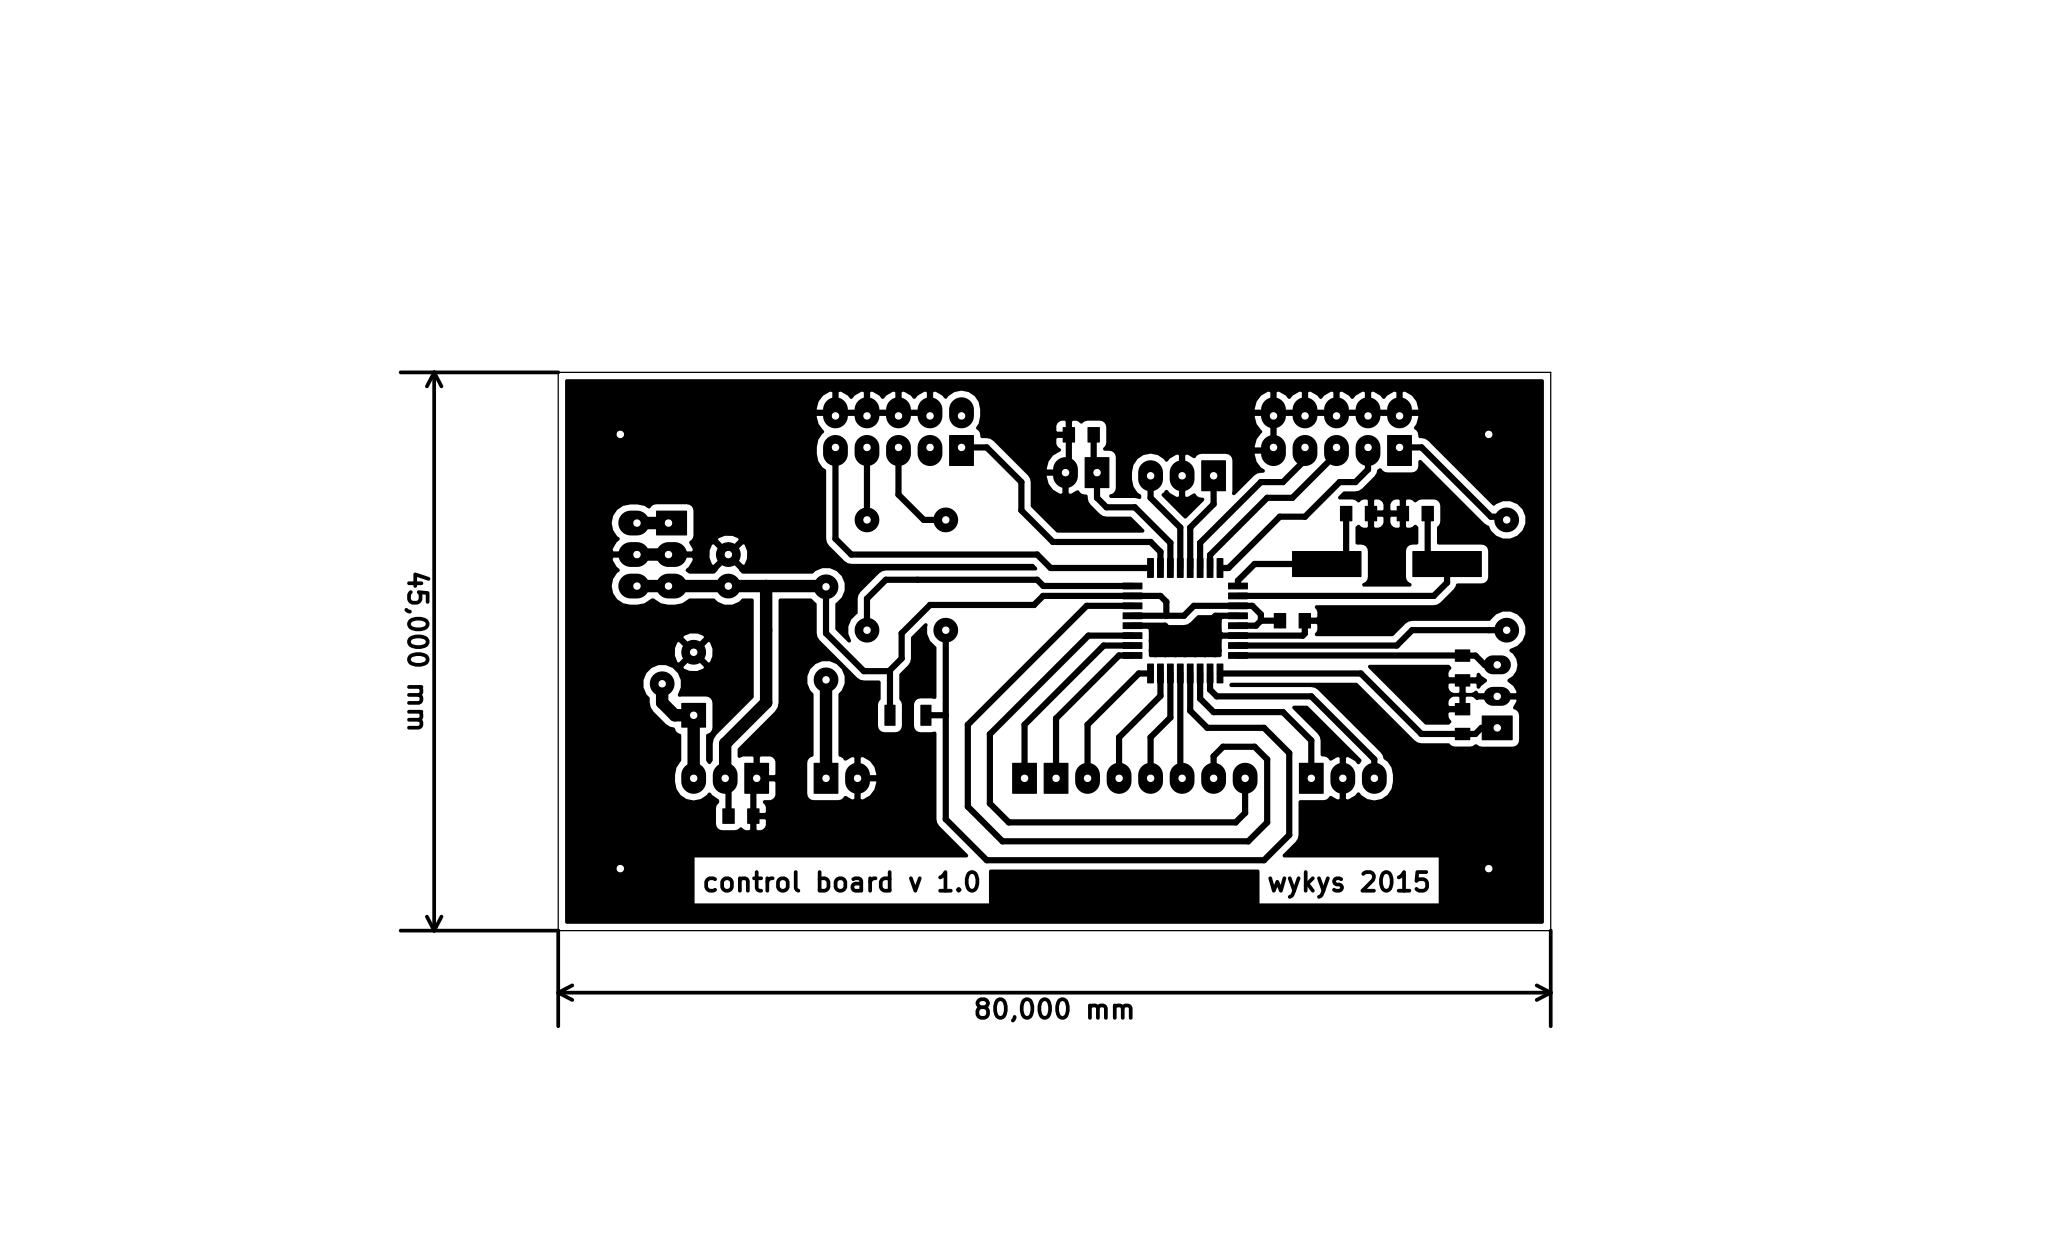
\includegraphics[width=170mm]{img/zdroj/cu_b.pdf}
	\caption{Deska plošného spoje zdroje napětí, strana spojů}    		
\end{figure}

% os f
\begin{figure}[H]
	\centering
	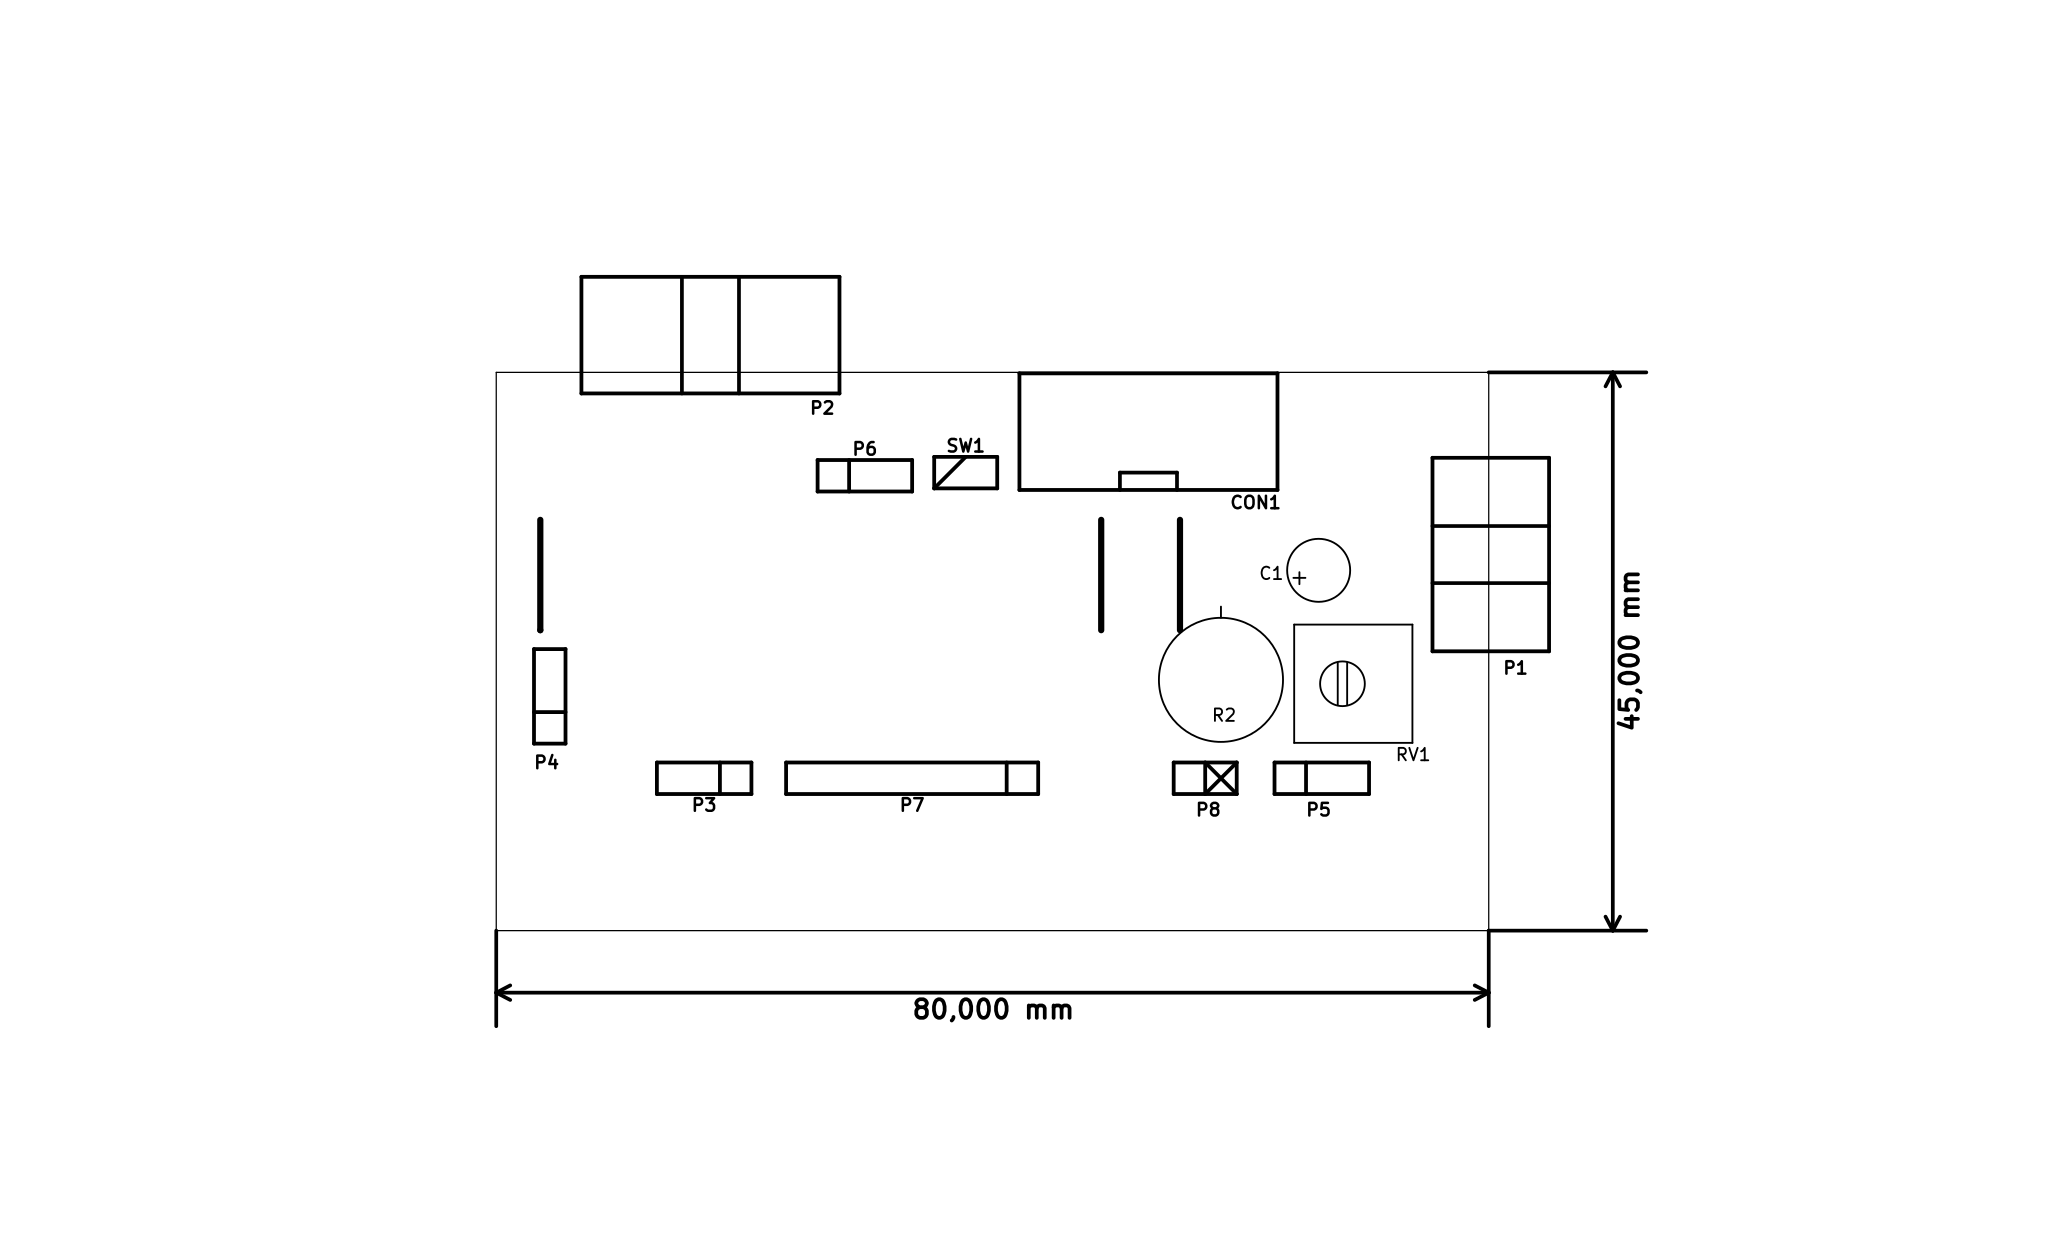
\includegraphics[width=170mm]{img/zdroj/os_f.pdf}
	\caption{Osazovací plán zdroje napětí, strana součástek}    		
\end{figure}

% os b
\begin{figure}[H]
	\centering
	
\includegraphics[width=170mm]{img/zdroj/os_b.pdf}
	\caption{Osazovací plán zdroje napětí, strana spojů}    		
\end{figure}